\documentclass[a4paper,openany,oneside,12pt]{book}
\usepackage[spanish]{babel}
\usepackage{graphicx}
\usepackage[utf8]{inputenc} % Para poner acentos y eñes directamente.
\usepackage{pdfpages}
\usepackage{listings}
\usepackage[T1]{fontenc}
\usepackage{hyperref}

\newcommand{\textsharp}{$\sharp$}

\begin{document}

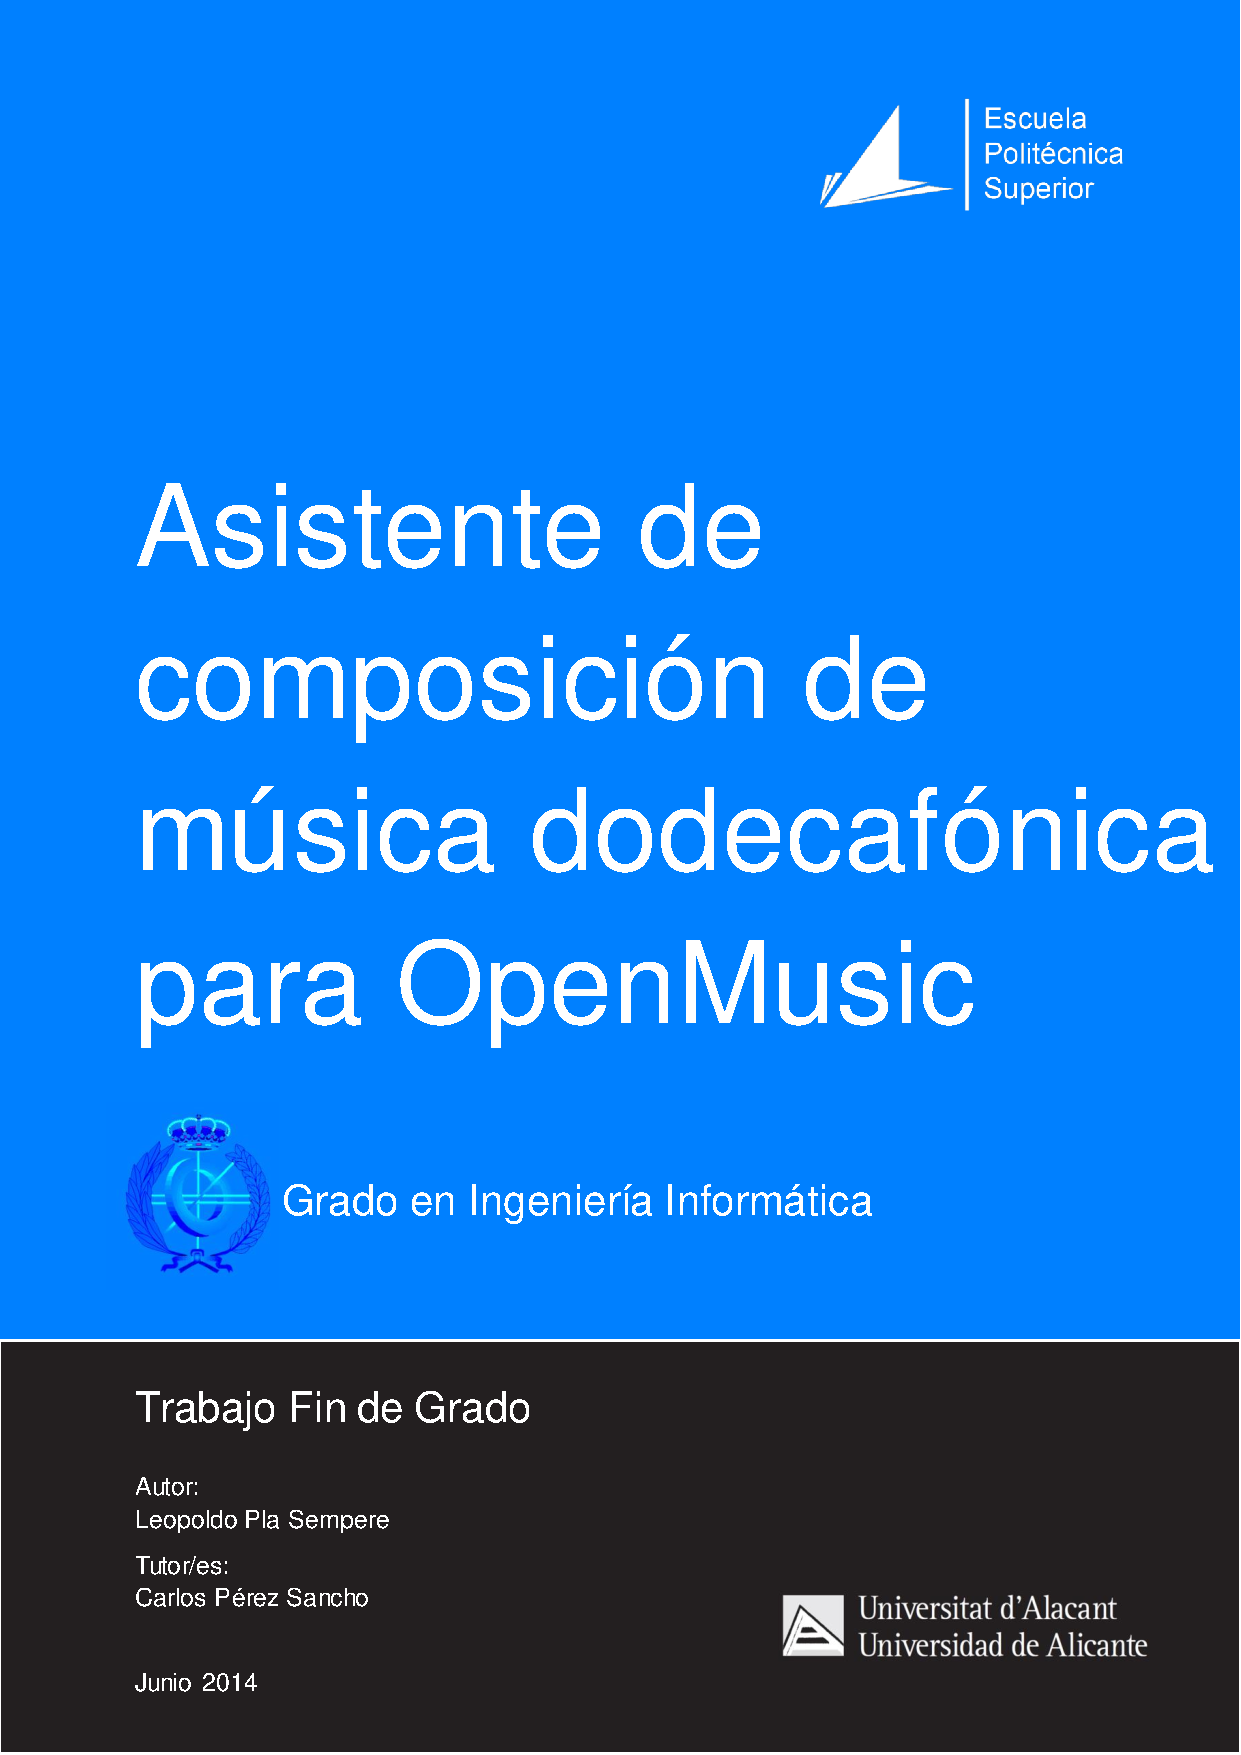
\includepdf[pages={1}]{img/Portada_GII.pdf}
\thispagestyle{empty} % para que no se numere esta pagina

\title{Asistente de composici\'on de m\'usica dodecaf\'onica para OpenMusic}
\author{
        Leopoldo Pla Sempere (lps34 at alu dot ua dot es)\\
        Universidad de Alicante\\
}

\date{\today}
\maketitle

\newpage
\mbox{}
\thispagestyle{empty} % para que no se numere esta pagina


\chapter*{Justificación y objetivos}
\pagenumbering{Roman} % para comenzar la numeracion de paginas en numeros romanos
La principal razón por la que he realizado este trabajo ha sido por aprovechar los conocimientos de los dos estudios realizados, el Grado Profesional de música y el Grado en Ingeniería Informática con especialidad en Computación en un proyecto que pueda ser útil para ambas áreas, ayudando a los músicos a componer y sentando una base para los ingenieros que quieran hacer un asistente de composición o que tengan ideas para mejorarlo. También una de las razones por la cuál he elegido esta área de la música como es la composición, y más concretamente el dodecafonismo, es la curiosidad sobre la programación en entornos de composición musical, la mejora e integración de los ordenadores en tareas mecánicas o programables como la composición de música dodecafónica y la relación de la música dodecafónica con el álgebra lineal.

El objetivo principal que se quiere alcanzar con este trabajo es, como he mencionado antes, mejorar el proceso de composición de música dodecafónica con una herramienta inédita proporcionando al compositor ideas y fragmentos generados con las restricciones que él desee así como retroalimentar al programa proponiendo más restricciones o formas compositivas que pueda crear para que otros ingenieros puedan mejorar este sistema.


\chapter*{Agradecimientos}
\addcontentsline{toc}{chapter}{Agradecimientos} % si queremos que aparezca en el índice
\markboth{AGRADECIMIENTOS}{AGRADECIMIENTOS} % encabezado
 
Agradecer este trabajo a mi familia por la ayuda y el apoyo que me han dado para llegar a crear este documento que mezcla dos mundos muchas veces duros de conllevar.

A mi tutor, Carlos, por orientar de una manera sencilla el proyecto y ser honesto con los objetivos propuestos.

A mis compañeros y profesores del grado, con los que he compartido muy buenos momentos y mucha experiencia profesional.

\chapter*{Licencia}
Documento liberado la licencia Creative Commons Attribution - ShareAlike 4.0 International (CC BY-SA)

\url{http://creativecommons.org/licenses/by-sa/4.0/}


\begin{figure}
\centering

\includegraphics{img/cc.png} 

This work is licensed under a Creative Commons Attribution-ShareAlike 4.0 International License.
\end{figure}

\chapter*{}
\begin{flushright}
\textit{Dedicado a \\
Laura}
\end{flushright}


\chapter*{Resumen}
\addcontentsline{toc}{section}{Resumen} % si queremos que aparezca en el índice
\markboth{RESUMEN}{RESUMEN} % encabezado

El asistente de composición de música dodecafónica es un conjunto de capas software implementadas sobre varias tecnologías, entre ellas OpenMusic y Python, para crear obras dodecafónicas según unas restricciones impuestas por el usuario. El sistema es capaz de obtener una serie dodecafónica en base a una semilla propuesta cumpliendo además ciertas restricciones para luego obtener todas las series derivadas de ella y componer con estas series y otras restricciones.

Se genera una partitura con ritmos, saltos de octava y silencios además de poder exportar el resultado a formato MusicXML para poder seguir editando en cualquier editor de partituras actual. Aquí presentaremos y mostraremos en imágenes el asistente con algunos ejemplos así como de exponer diferentes partes de su desarrollo. También se mostrará la estructura y la programación del programa bajo las diferentes tecnologías utilizadas y se sugieren enfoques para el futuro desarrollo.



\newpage


\tableofcontents % indice de contenidos

\cleardoublepage
\addcontentsline{toc}{chapter}{Lista de figuras} % para que aparezca en el indice de contenidos
\listoffigures % indice de figuras





\chapter{Introduction}
\pagenumbering{arabic} % para empezar la numeración con números
Con el avance del procesamiento de la información, han surgido herramientas para músicos que ayudan a realizar tareas tanto a nivel de tratamiento del sonido, edición y síntesis como a nivel de aprendizaje musical y rítmico, abarcando tanto a músicos aficionados o profesionales como a ingenieros de diversas ramas. Una de las vías que mantiene unidos a los músicos profesionales y los ingenieros es la música por ordenador (o la representación musical), donde los grupos que tratan esta materia investigan y desarrollan estructuras, lenguajes y paradigmas adaptados a la música.

Las áreas que más se tratan en estos grupos actualmente son la clasificación de música, análisis y composición automática (siendo esta la que más tiempo se lleva investigando y desarrollando). Todas estas áreas de la música conllevan el conocimiento de técnicas como el reconocimiento de patrones (\emph{pattern recognition}) o el aprendizaje máquina (\emph{machine learning}). Desarrollaremos en este trabajo la asistencia para la composición de obras dodecafónicas por ordenador, aún no desarrollada en el ámbito de la composición automática.

\chapter{Marco teórico y tecnologías utilizadas}\label{marcoteorico}
\section{Dodecafonismo}

Arnold Schoenberg (1874-1951) fue un compositor, teórico musical y pinto austriaco de origen judío. En 1905 creó un método de composición basado en la ausencia de centro tonal, el atonalismo, ya que para Arnold la tonalidad era un recurso que se había explotado al máximo y se debía buscar alternativas armónicas para la composición. Este método aumentó la dificultad de composición de obras extensas ya que era muy limitado para crear estructuras coherentes de larga duración sin que estuviesen apoyadas en un texto que las cohesionase. Este movivo provocó que entre 1914 y 1921 no publicara ningún escrito hasta que creó una solución. Entre 1921 y 1923 inició un método de composición musical derivado del atonalismo que solventaba sus limitaciones: el dodecafonismo (\emph{twelve-tone method})\cite{styleandidea}. La primera obra que publicó con este método es la Suite para piano Op. 25.

Schoenberg creó este método por el mismo hecho histórico por el que se pasó de la música modal a la música tonal: por el desarrollo natural e histórico de la música.

\begin{quote}
\em Este compromiso que se llama 'sistema temperado', representa una tregua por un tiempo indeterminado. Pues esta reducción de las relaciones naturales a las manejables no podrá resistir indefinidamente la evolución musical; y cuando el oído lo exija se enfrentará con el problema. Y entonces nuestra escala quedará asumida en una ordenación superior, como lo fueron los modos eclesiásticos en los modos mayor y menor. Y no podemos prever si habrá cuartos, octavos, tercios de tono o (como piensa Busoni) sextos de tono, o si iremos directamente a una escala de 53 sonidos como la establecida por el Dr. Robert Neuman.\cite{tratadodearmonia}
\end{quote}

Este método de composición es un tipo de serialismo (composición basada en series de notas, de ritmos, de dinámicas...) en el que no se busca la importancia de unas notas sobre otras (que es la base de la tonalidad). Es decir, busca lo contrario que la música tonal (por ejemplo, la música clásica, o la música rock), que tiene normalmente un tono predominante y unas notas dominantes sobre otras (la dominante sobre la tónica, que definen el tono y crea centros tonales). Para evitar este énfasis, se crea una serie con las doce notas de la escala cromática  sin repetirse ninguna, de forma que se les da la misma importancia, se crean series derivadas, y se compone solamente con estas construcciones \cite{wiki:twelvetonetechnique}. Esta forma de componer crea, pues, atonalidad pero mantiene una razón para la estructura que son las series. 

Para componer con el método dodecafonista primero se ha de obtener, como hemos dicho anteriormente, una matriz donde la primera fila es la serie original (las 12 notas de la escala cromática en un orden) y la primera columna es la serie invertida (serie construida por movimiento contrario de la serie original, es decir, si la primera nota es un Do y la segunda un Re en la serie original, en la invertida será un Do y un Si). Si leemos la fila y columna al contrario (de izquierda a derecha o de abajo a arriba respectivamente) obtenemos la serie retrógrada y la serie retrógrada inversa en cada caso. El resto de elementos de la matriz se puede obtener transportando en base a los elementos de la primera fila o la primera columna.

En la figura \ref{fig:matrix} vemos un ejemplo. La primera fila de la matriz es la serie original (Do, Do\textsharp, Re, Si, La\textsharp, Sol\textsharp, Mi, La, Re\textsharp, Fa\textsharp, Fa, Sol) y que la serie inversa se obtiene leyéndola de derecha a izquierda: Sol, Fa, Fa\textsharp, Re\textsharp, La, Mi, Sol\textsharp, La\textsharp, Si, Re, Do\textsharp, Do). Para obtener la primera columna vemos que la distancia del primer elemento con el segundo es un semitono ascendente (de Do a Do\textsharp), con lo que el segundo elemento de la serie inversa será un Si, es decir, un semitono descendente. Exactamente igual con el tercer elemento, en el que del segundo elemento al tercero de la serie original (Do\textsharp y Re) hay otro semitono ascendente, con lo que en la serie invertida, será un semitono descendente respecto al segundo elemento de la serie inversa (Si), por lo que la serie por ahora sería: Do, Si, La\textsharp. Si continuamos con este procedimiento obtenemos la serie inversa: Do, Si, La\textsharp, Do\textsharp Re, Mi, Sol\textsharp, Re\textsharp, La, Fa\textsharp, Sol, Fa. 

La numeración se basa en el número de la nota: 0 es Do, 1 es Do\textsharp, 2 es Re... Y P es la serie original, R la retrógrada, I la inversa y RI es la retrógrada inversa. Para el resto de matriz, transportamos verticalmente o horizontalmente. Si lo hacemos horizontalmente, vemos que como del primer elemento al segundo hay un semitono descendente (de Do a Si), transportamos todos los elementos de la serie original un semitono hacia abajo. En la tercera fila se puede basar en la que acabamos de obtener o en la serie base, el transporte es diferente pero el resultado es el mismo.

Un ejemplo muy claro de una obra dodecafónica se puede ver en este PDF cortesía de Dan Román del Conservatorio de Música de Puerto Rico: \url{http://musike.cmpr.edu/v001/roman-eng.pdf}

\begin{figure}
\centering
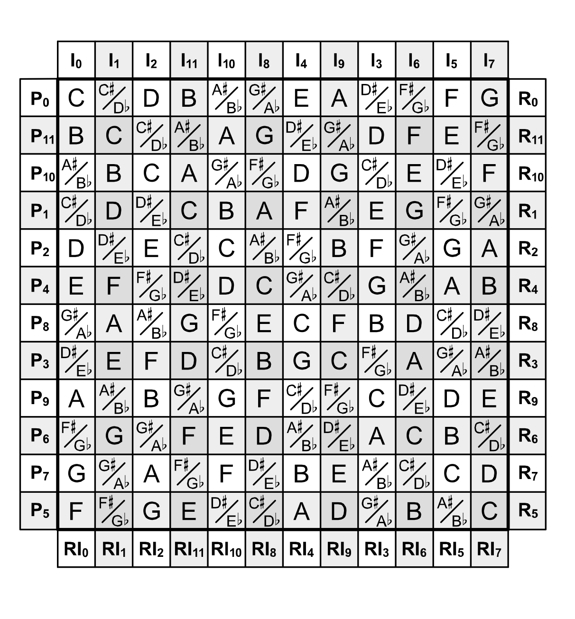
\includegraphics[width=0.8\textwidth]{img/12_tone_matrix.jpg} 
\caption{Matriz dodecafónica. \cite{musictheory}} \label{fig:matrix}
\end{figure}

\begin{quote}
\em Expuesto de esta manera, el método puede parecer arbitrario. Pero para Schönberg, se trataba de un modo sistemático de llevar a cabo lo que ya estaba haciendo en su música tonal: integrar la armonía y la melodía mediante la composición con un número limitado de conjuntos (aquí, los definidos por los segmentos de la serie), delimitar las frases y subfrases por medio de la saturación cromática (regulada por la aparición de las doce notas en cada exposición de la serie) y apoyarse en la variación en desarrollo. \cite{palisca}
\end{quote}

\section{Backtracking}
\begin{quote}

\em Vuelta atrás, (Backtracking) es una estrategia para encontrar soluciones a problemas que satisfacen restricciones. El término fue acuñado por primera vez por el matemático estadounidense D. H. Lehmer en la década de 1950. 

En su forma básica, la idea de backtracking se asemeja a un recorrido en profundidad dentro de un grafo dirigido. El grafo en cuestión suele ser un árbol, o por lo menos no contiene ciclos. Sea cual sea su estructura, existe sólo implícitamente. El objetivo del recorrido es encontrar soluciones para algún problema. Esto se consigue construyendo soluciones parciales a medida que progresa el recorrido; estas soluciones parciales limitan las regiones en las que se puede encontrar una solución completa. El recorrido tiene éxito si, procediendo de esta forma, se puede definir por completo una solución. En este caso el algoritmo puede, o bien detenerse (si lo único que se necesita es una solución del problema) o bien seguir buscando soluciones alternativas (si deseamos examinarlas todas). Por otra parte, el recorrido no tiene éxito si en alguna etapa la solución parcial construida hasta el momento no se puede completar. En tal caso, el recorrido vuelve atrás exactamente igual que en un recorrido en profundidad, eliminando sobre la marcha los elementos que se hubieran añadido en cada fase. Cuando vuelve a un nodo que tiene uno o más vecinos sin explorar, prosigue el recorrido de una solución. \cite{wiki:backtracking}


\begin{figure}
\centering
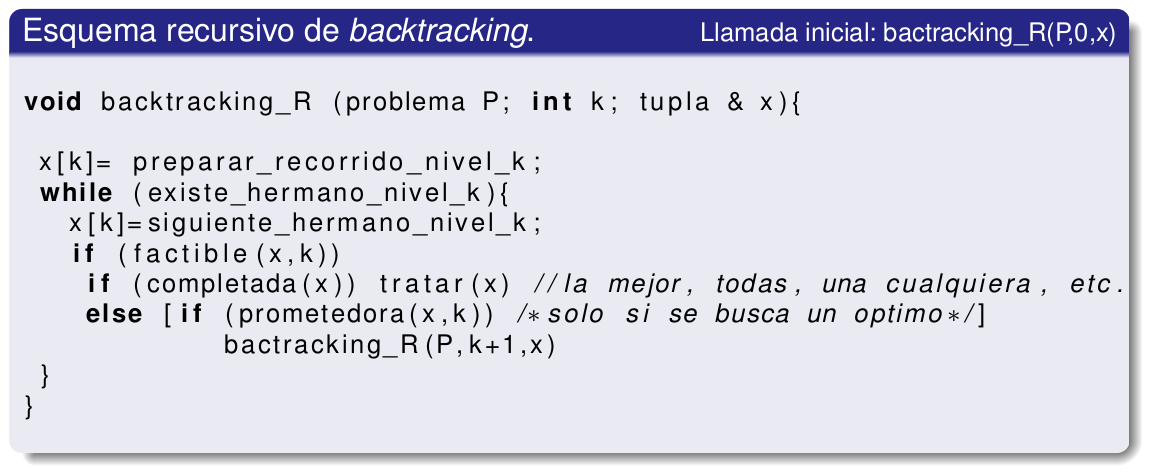
\includegraphics[width=\textwidth]{img/backtracking.png}
\caption{Esquema recursivo del backtracking, apuntes de la asignatura Análisis y Diseño de Algoritmos} \label{fig:backtracking}
\end{figure}


\end{quote}
\section{OpenMusic}

OpenMusic \cite{openmusic} es un entorno de programación visual orientado a objetos basado en Common Lisp. Se puede utilizar como entorno de programación visual para programación en Lisp ya que implementa la mayoría de construcciones del lenguaje Common Lisp (condicionales, bucles o gestión de listas). Además de añadir un conjunto de estructuras y objetos musicales como acordes, secuencias de acordes, ritmos... Tamién incluye herramientas de reproducción MIDI, análisis de ficheros de sonido, representación de objetos 3D...

Este entorno fue diseñado en el IRCAM (Institut de Recherche et Coordination Acoustique/Musique) en 1998 y lanzado bajo licencia LGPL. Funciona bajo Windows, OS X y en los últimos meses se han empezado a publicar versiones para GNU/Linux.

\begin{figure}
\centering
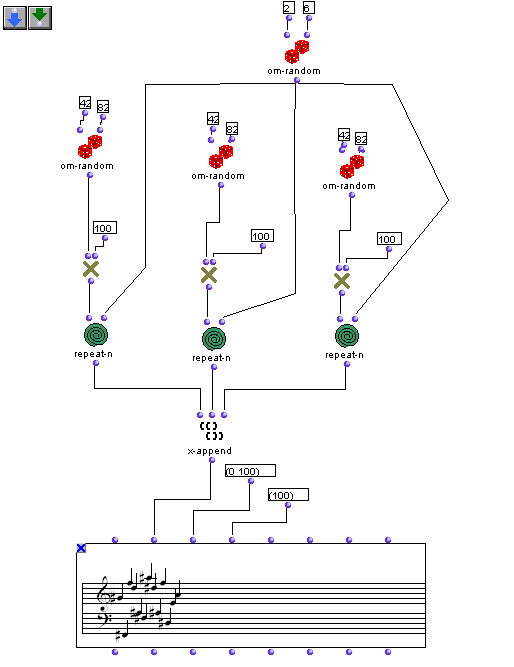
\includegraphics[width=0.8\textwidth]{img/Om_patch.png} 
\caption{Ejemplo de programa escrito en OpenMusic. \cite{wiki:openmusic}} \label{fig:openmusic}
\end{figure}


Los siguientes compositores han reconocido utilizar OpenMusic \cite{wiki:openmusic}:

\begin{itemize}
\item Alain Bancquart
\item Brian Ferneyhough
\item Joshua Fineberg
\item Karim Haddad
\item Eres Holz
\item Michael Jarrell
\item Fabien Lévy
\item Fang Man
\item Philippe Manoury
\item Tristan Murail
\item Kaija Saariaho
\item Marco Stroppa
\end{itemize}

Además de poder programar de forma visual, al estar basado en Common Lisp, se permite crear funciones escritas en código y ser utilizadas en el entorno visual.
\section{Lisp}
Lisp es una familia de lenguajes de programación multiparadigma basados en listas y con notación basada en paréntesis creada por John McCarthy en 1958 en el MIT (Massachusetts Institute of Technology). El nombre de LISP deriva de ``LISt Processing'', dado que la estructura más importante del lenguaje es la lista (el código fuente de Lisp está compuesto por listas).\cite{wiki:lisp} Se popularizó en los entornos de la inteligencia artificial y fue pionero en conceptos de la ciencia de la computación como las estructuras de árboles o los tipos dinámicos.

Es el segundo lenguaje de alto nivel más viejo con alto uso hoy en día, por detrás de FORTRAN. Los dialectos más conocidos de esta familia son Scheme y Common Lisp.

La sintaxis del código se basa en expresiones S, donde el primer elemento después del paréntesis izquierdo es el nombre de la función y el resto de elementos son los argumentos. Por ejemplo:

\lstset{language=Lisp}
\begin{lstlisting}
(+ 1 3 (* 4 5))
; Output: 24
\end{lstlisting}


\subsection{Common Lisp}
Common Lisp es un dialecto de Lisp estandarizado por la ANSI (American National Standards Institute) creado para estandarizar las variantes de Lisp. Es un lenguaje de propósito general y multiparadigma: combina los paradigmas procedural, funcional y orientada a objetos. Al ser un lenguaje dinámico (los comportamientos del lenguaje se producen en tiempo de ejecución) facilita el desarrollo de software de forma incremental. Existen diferentes implementaciones del estándar, tanto de código abierto como propietarios. \cite{wiki:commonlisp} 

En comparación con el otro dialecto más famoso de Lisp, Scheme, las diferencias vienen dadas por algún cambio mínimo en la sintaxis (las declaraciones de funciones con defun dejan el nombre de la función fuera de la lista de argumentos en Common Lisp y en Scheme dentro de la lista, por ejemplo), soporte para diferentes tipos de números (Common Lisp soporta racionales, punto flotantes, enteros con precisión arbitraria... En cambio Scheme como mucho soporta números en coma flotante) y optimizaciones a nivel de la cola de recursión o del tamaño del código del lenguaje.

\section{Python}
Es un lenguaje de programación interpretado, multiparadigma (orientado a objetos, imperativo y funcional), tipado débil, multiplataforma y de código abierto (Licencia PSFL). La filosofía de este lenguaje es la de una sintaxis preparada para hacer un código legible y sencillo.

\section{QT}
QT es un framework para aplicaciones multiplataforma utilizado para el desarrollo de interfaces gráficas en proyectos software o también programas sin interfaz para consola y consolas para servidores. También es software libre (bajo licencia GPLv3). El proyecto se hizo famoso en el desarrollo del entorno KDE y con el desarrollo de empresas como Nokia.

\section{PyQt}
La unión de los dos proyectos anteriores se conoce como PyQt4, que aprovecha el conjunto de clases de Qt para crear una interfaz y las herramientas de diseño que incorpora y la simplicidad y posibilidad del uso de objetos del código de Python, además de ser un lenguaje que no necesita un ciclo de \emph{edición/compilación/linkeado/ejecución} que aumenta la productividad. Además, como las dos herramientas en las que está basado el proyecto es multiplataforma, lo convierte también en multiplataforma. Todo este conjunto de características hace que sea el complemento perfecto para crear interfaces y scripts rápidos para programas de OpenMusic.


\chapter{Cuerpo del trabajo}\label{cuerpo}
\section{Esquema del sistema}
El asistente de composición de música dodecafónica viene estructurado por 5 capas de software: la interfaz con Qt4, el script de generación de parámetros en Python3, el ``patch'' (en adelante programa) en OpenMusic (mayoritariamente código de Common Lisp) para la generación de la serie, el programa en OpenMusic para la generación de la partitura en OpenMusic y la visualización de la partitura completa en un visor externo (ya desarrollado, como puede ser Finale Notepad, que es gratuito y compatible con la versión del formato MusicXML que exporta OpenMusic).

\begin{figure}
\centering
\noindent\makebox[\textwidth]{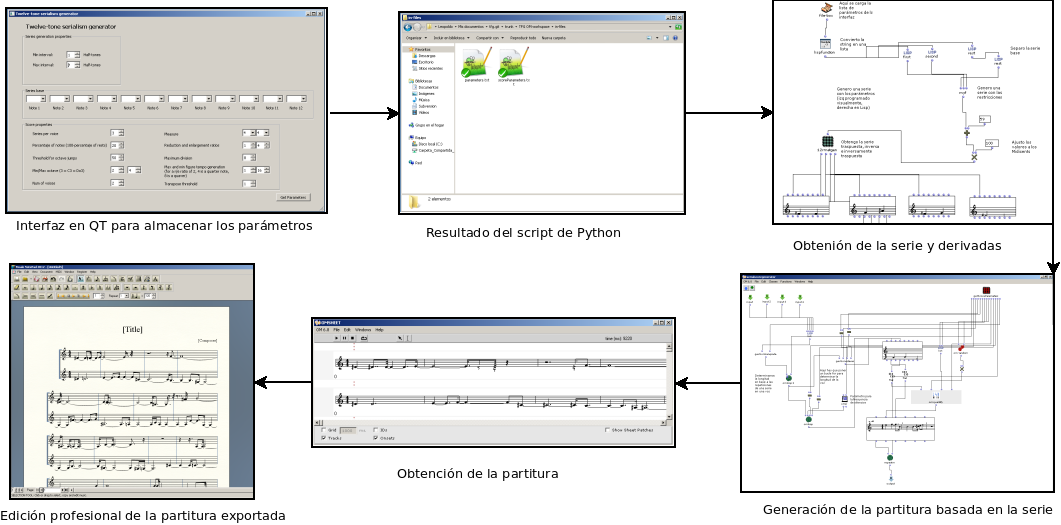
\includegraphics[width=0.9\paperwidth]{img/software_diagram.png}}
\caption{Diagrama del diseño del asistente.} \label{fig:softwarediagram}
\end{figure}

\subsection{Interfaz gráfica}

La interfaz en Qt4 se ha diseñado utilizando Qt4 Designer, herramienta incluida en la instalación de Qt4 en el sistema y que permite utilizar todas las herramientas de Qt4 en un editor ``click and drop'', pudiendo ver el resultado de la interfaz sin siquiera saber bajo qué código se va a ejecutar.

\begin{figure}
\centering
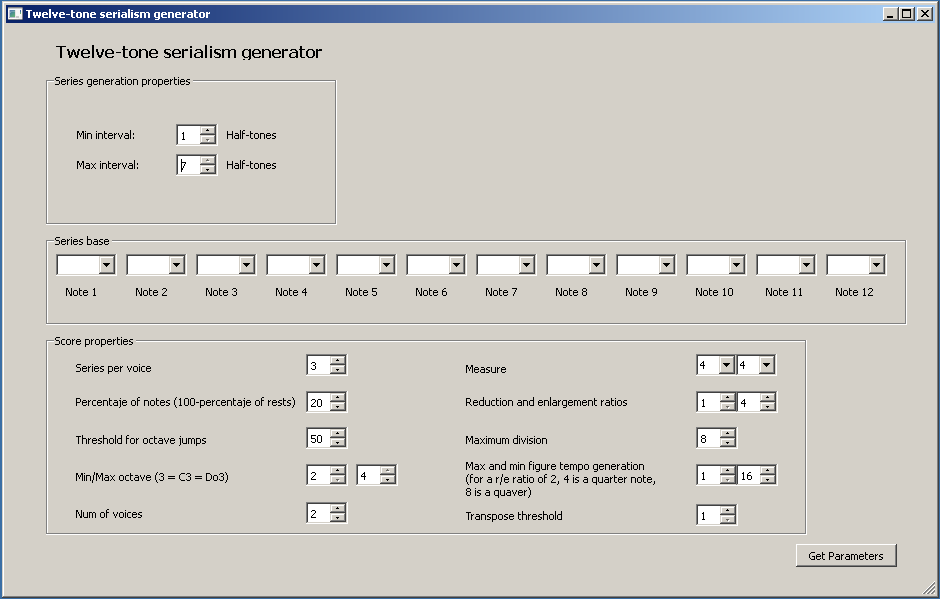
\includegraphics[width=\textwidth]{img/qtprogram.png}
\caption{Interfaz en Qt bajo Windows 7} \label{fig:qtinterface}
\end{figure}

El fichero que se obtiene del editor Qt4 Designer es un .ui, que con la herramienta pyuic4 (Python-UI converter 4) convertimos el fichero .ui obtenido en un fichero de Python. Dado que la herramienta pyuic4 muestra por pantalla el resultado, se ha de ejecutar con el símbolo ``>'' después del argumento del fichero a convertir para guardarlo en un fichero .py. El comando en Windows es (suponiendo que estamos en la carpeta con los 2 ficheros a utilizar):

   \lstset{language=Bash,
           basicstyle=\ttfamily\scriptsize,
           keywordstyle=\ttfamily,
           stringstyle=\ttfamily,
           commentstyle=\ttfamily,
          breaklines=true
          }
\begin{lstlisting}
pyuic4.bat RuleTranslator.ui > RuleTranslatorInterface.py
\end{lstlisting}

Este fichero es cargado por el script en Python y se le llama con las directivas propias de Qt4 en Python3. Carga la interfaz, convierte los valores de la interfaz en números y los agrupa en forma de lista antes de exportarlos a dos ficheros de texto para que OpenMusic los pueda abrir y procesar. En el código fuente se puede ver claramente cómo funciona este sencillo script.

\subsection{Generador de series}
Una vez hemos obtenido los parámetros del compositor, se cargan con el método de lectura de ficheros de OpenMusic y se convierten con un método de Lisp llamado \emph{read-from-string}. El método encargado de la generación de la serie basándose en las restricciones de mínimo y máximo salto de semitonos y en la serie semilla (introducidos por la interfaz) es el método escrito en Common Lisp \emph{seriesGenerator} (empaquetado en forma de librería para hacerlo más accesible y reutilizable en otros proyectos).

Este código ha sido diseñado para obtener una solución siempre que sea posible dadas las restricciones utilizando backtracking en una implementación recursiva. El esquema del algoritmo diseñado es:

   \lstset{language=Lisp,
           basicstyle=\ttfamily\scriptsize,
           keywordstyle=\ttfamily,
           stringstyle=\ttfamily,
           commentstyle=\ttfamily,
          breaklines=true
          }
\begin{lstlisting}
    ; Obtiene las notas que faltan en la secuencia parcial y las guarda en una lista llamada notasfaltan

    ; reordenar aleatoriamente notasfaltan

  	; para cada elemento de notasfaltan iteramos (bucle)
      ; Creamos una copia para no modificar la lista original
      ; seleccionar nueva nota y comprobamos si cumple las restricciones
      ; obtener posicion del primer cero (elemento a rellenar en la semilla)
      ; en la posicion -1 esta la nota anterior
      
      ; Si es la primera posicion de la lista no se mira el elemento anterior porque no hay
          ; llama recursivamente a seriesGenerator con la nueva lista
          ; si seriesGenerator devuelve una lista completa entonces termina el bucle y devuelve la lista


          ; Si no es la primera posicion de la lista, miramos las restricciones respecto a la nota anterior
              ; si las dos notas cumplen las restricciones, asigna la nueva nota en la posicion del primer cero (hueco en la semilla)
              ; llama recursivamente a seriesGenerator con la nueva lista
              ; si seriesGenerator devuelve una lista completa entonces termina y devuelve la lista




  ; si al terminar el bucle ninguna nota cumple la restriccion devuelve lista vacia

\end{lstlisting}

Dado que cualquier solución que cumpla las condiciones nos sirve, no recorremos todo el árbol, tan sólo nos desplazamos por el árbol hasta encontrar la primera solución posible.

Para poder ver la implementación en Lisp, abrir el fichero \emph{serieGenerator.lisp} en la librería \emph{twelvetonelib 1.0} dentro del ``workspace'', donde están los fuentes de todos los métodos implementados en Lisp.

Obtenida la serie con este código, procedemos a computar las 4 series básicas (sin trasporte) de la matriz dodecafónica: P, I, R, RI.

La serie P la obtenemos del método anterior y la inversa se obtiene aplicando el método \emph{reverse} de Lisp. Para obtener la serie retrógrada programamos el mismo proceso que el manual.

Existen dos métodos en OpenMusic llamados x->dx y dx->x que devuelven una lista de intervalos de una lista de notas y viceversa. Es decir, si a x->dx se le pasan los valores de las notas en midicents 2000, 2500, 3200 devuelve (500 700), y si a dx->x le pasamos una nota (por ejemplo 1500) y los valores obtenidos con el ejemplo de antes (500 700), obtenemos (1500 2000 2700).

Si multiplicamos por -1 el valor de los intervalos (tal y como hacemos a mano, ya que si un intervalo es de X semitonos ascendente en la serie original, la inversa son X semitonos descendente) obtenemos la serie inversa y si le aplicamos el método \emph{reverse} tenemos la retrógrada inversa.

Este proceso está programado en un ``patch'' de OpenMusic dado que visualmente es sencillo de programar. En el proyecto de OM se llama \emph{12rmatgen}.

\subsection{Generación de la partitura}
En la generación de una partitura intervienen restricciones introducidas en la interfaz: 
\begin{itemize}
\item número de series que aparecen en una voz (determinando en parte su longitud)
\item porcentaje de notas (para generar también silencios)
\item \emph{threshold} para cambiar de octava (para saltar desde muy rápidamente a muy lentamente)
\item octavas máximas y mínimas (desde Do2 hasta Do4)
\item número de voces de la partitura, compás (2/4, 3/4, 4/4, 3/8, 6/8, 2/1...)
\item máximo y mínimo valor para la reducción y ampliación (sirve para que el compositor pueda bloquear una voz ya generada y ver cómo puede quedar reduciendo o ampliando los tamaños de las notas)
\item división máxima (siendo 8 la semicorchea, 4 la corchea, 2 la negra...)
\item dimensión de las figuras máximas y mínimas (para un valor de factor de aplicación y reducción de 2, 4 es una corchea, 8 es una negra...)
\item un threshold para el transporte (a mayor valor, menos transporte se utiliza, es decir, más se utilizan las series básicas P, I, R, RI).
\end{itemize}

Estos parámetros se cargan de forma similar que con las restricciones de la serie, sólo que aquí, dado que son 14 parámetros, se ha decidido por crear un ``patch'' interno (un subprograma) dentro del ``patch'' que genera la partitura (\emph{serialscoregenerator}).

La generación de la partitura se procesa a través de varias fases. Partimos de las 4 series generadas con \emph{12rmatgen} (P, I, R, RI). Primero vamos a determinar la longitud de la voz, es decir, cuántas series va a tener una voz. De manera que si una voz tiene dos series, esa voz tendrá una longitud de 24 notas (luego se le añadirán silencios o no y se pondrá un compás y una longitud a esas notas).

En el bucle \emph{longitud y transporte} iteramos tantas veces como se le haya asignado por parámetro, eligiendo una de las series de la matriz de forma aleatoria. El resultado le llega al siguiente bucle que calcula la longitud de las notas. Itera para cada una de las notas de la voz y les asigna un valor de longitud entre los valores pasados por parámetro. Además, con el threshold de silencios, en el caso en el que la función random pase ese threshold, la longitud de la nota será negativa (si el valor 1000 para la duración es una figura de negra, un valor de -1000 es un silencio de negra).

Una vez con la listas de valores de midicents para la voz y de duraciones de las notas, pasamos la lista de duraciones a un objeto característico de OpenMusic: \emph{omquantify}.

Este método se encarga convertir duraciones en milisegundos (tal y como tenemos en la lista de duraciones) en una medida dentro de un compás. Si vemos en el código del generador de partituras, hay dos visualizaciones de los resultados: una sin compás y donde todas las notas son negras (con separaciones diferentes) y una muy cercana a una partitura final.

\begin{figure}
\centering
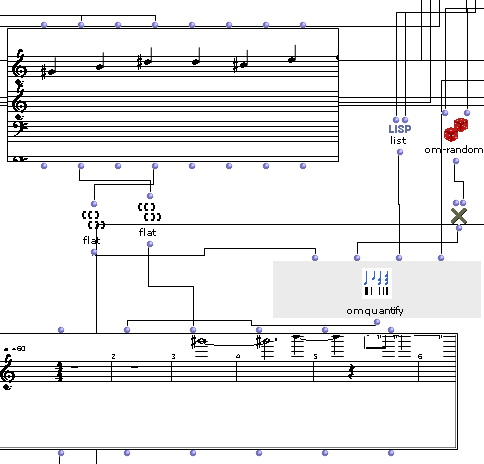
\includegraphics[width=0.7\textwidth]{img/visores.png}
\caption{Distintas visualizaciones de listas de midicents y duraciones} \label{fig:visores}
\end{figure}

El método \emph{omquantify} recibe cuatro parámetros: la lista de duraciones, el tempo, el compás y la mínima división posible. Estos tres últimos parámetros se leen del fichero obtenido de la interfaz. El tempo hace que una misma duración de una nota se interprete como una nota más larga o más corta. Por ello, se ha interpretado en la interfaz como valor de reducción y ampliación, porque para una misma voz, un valor más alto de reducción y ampliación genera la misma voz pero más larga. La mínima subdivisión se establece porque como es un método que traduce milisegundos a medición musical, si establecemos un valor muy bajo, para fluctuaciones irregulares (por ejemplo, un tempo de negra igual a 60), si tenemos 1002 milisegundos, podría generar fusas, semifusas o valores incluso más bajos (ya que una negra es 1000 ms) y con este valor se pueden corregir esas fluctuaciones.

Finalmente, una vez se haya cuantificado el valor de los tiempos en medición musical, obtenemos un objeto \emph{voice} con esta cuantificación y las notas en midicents. Iteramos tantas veces como voces hayamos especificado y devolvemos el valor a un objeto \emph{score} donde se puede reproducir y editar de forma limitada. También se llama al bucle para exportar para poder visualizarlo en programas profesionales de edición de partituras.


\subsection{Uso de los ficheros exportados}
Dadas las limitaciones de OpenMusic y su método de exportación a XML, sólo permite exportar voces individuales a XML, no objetos \emph{score} directamente. Por ello, vemos los ficheros de cada voz exportados en la carpeta \emph{out-files} del workspace. El programa que oficialmente da soporte OpenMusic con XML es Finale. 

Finale es un software propietario de pago para la edición de partituras, pero dispone de un visualizador y editor simple (más avanzado aún así que el editor de partituras de OpenMusic) llamado Finale NotePad. 

En este programa, en el menú \emph{File/MusicXML/Import...} podemos abrir los ficheros y unir todas las voces en una sola partitura creando un nuevo proyecto y moviendo las partituras importadas a las voces del nuevo proyecto.

\begin{figure}
\centering
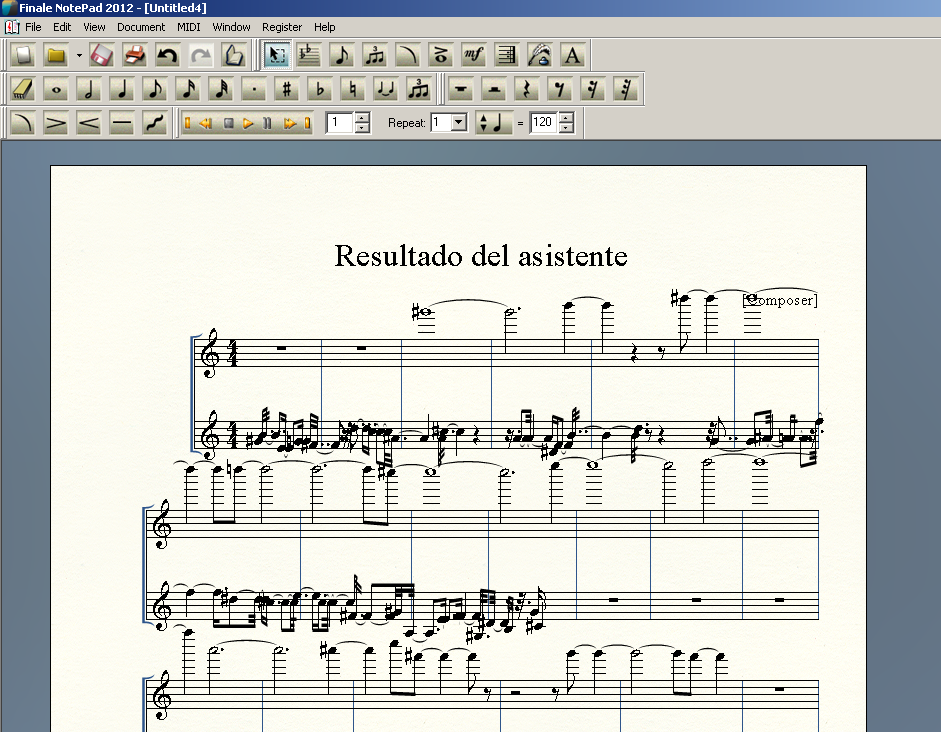
\includegraphics[width=0.8\textwidth]{img/finale.png}
\caption{Visualización del ejemplo en Finale} \label{fig:finale}
\end{figure}

Una vez tenemos el proyecto como tenemos mostrado, podemos seguir utilizando el asistente para que nos siga generando ideas acordes con lo que queremos, además aprovechando una de las características de la interfaz de OpenMusic, que es poder bloquear ciertos objetos para que no se vuelvan a calcular. Es decir, por ejemplo, si hemos generado una partitura con una serie que nos satisface, podemos bloquear el objeto de generación de series pulsando sobre él y pulsando la tecla \emph{b} del teclado para que se quede la evaluación previa (aparecerá una X en la esquina superior izquierda del objeto).

Finalmente, si quisiéramos exportar este fichero a otro editor con una versión (aquí sí compatible) de MusicXML 3.0 o en fichero MIDI, exportamos o guardamos (respectivamente) y podemos trabajar en el contexto que estemos acostrumbrados a trabajar con partituras.


\begin{figure}
\centering
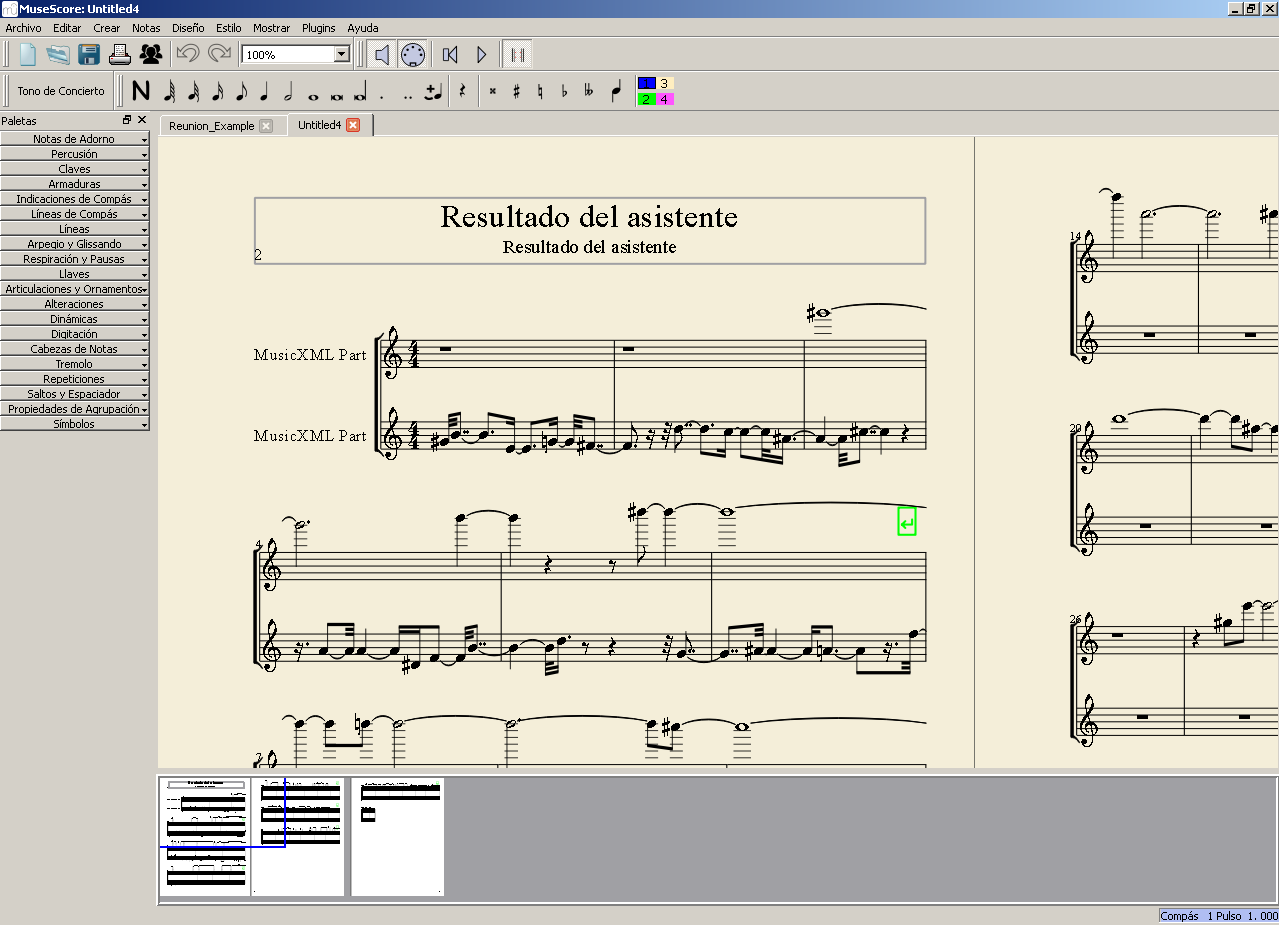
\includegraphics[width=0.9\textwidth]{img/musescore.png}
\caption{Visualización final del ejemplo en MuseScore} \label{fig:musescore}
\end{figure}

\chapter{Conclusiones}\label{conclusiones}
Tras haber probado el asistente bajo varias condiciones y diferentes parámetros, los resultados son satisfactorios, ya que se ha obtenido ayuda e ideas muy interesantes, con lo que se ha obtenido una herramienta musical informatizada complementaria para compositores. El objetivo de conseguir una herramienta que asiste a un músico a componer se ha conseguido aunque se pueden mejorar ciertos aspectos.

El desarrollo de este sistema se ha basado en un modelo incremental, de forma que partíamos de una especificación del proyecto y se ha ido modificando el conjunto de características según avanzamos en los ``sprints'' o hitos a lo largo del cuatrimestre. Se han realizado reuniones con el tutor para enfocar estos hitos y los diferentes prototipos del proyecto hasta conseguir el prototipo final.

Durante el desarrollo de este proyecto han surgido varios problemas de implementación dada la poca experiencia con OpenMusic, haciéndome ver las limitaciones que este programa tiene. El primer planteamiento fue el de implementar el método de generación de series dodecafónicas de forma visual. De hecho, hay gran parte implementado, pero a la hora de programar recursiones, la interfaz da muchos problemas y es mucho más difícil de conseguir que programándolo en Common Lisp. El ``patch'' que se inició a programar también está incluido en el proyecto y se llama \emph{seriegenerator}.

Otro problema existe con el tratamiento de MusicXML. Este estándar para la visualización y guardado de partituras tiene diferentes versiones. OpenMusic tiene implementada una versión antigua de forma que muchos de los editores de partituras no aceptan. En su página (y como hemos demostrado en el ejemplo) recomiendan Finale, y desde ahí, se permite exportarlo a unos formatos con implementaciones más actualizadas. También ha habido problemas de compatibilidad probando versiones más actualizadas de PyQT (como es PyQT5) pero da problemas con algunos elementos de la interfaz como las señales de activación de funciones, con lo que se decidió utilizar PyQT4, que es más estable.

Durante el desarrollo del proyecto han surgido ideas (tanto programando, como leyendo documentación como hablando con otros músicos) para mejorar el proyecto a largo plazo. Entre esas ideas, existe la posibilidad de programar formas compositivas barrocas y clásicas (estructura A-B-A, contrapuntos por ampliación, reducción, cánon...), desarrollar las series entre voces (es decir, la primera voz puede tener la mitad de una serie y la segunda la otra mitad como se puede ver en la imagen \ref{fig:twelvetoneexample}).

La mayoría de estos métodos implicaría refactorizar el método actual de construcción de partituras, que se basa en generar voces independientes únicamente mirando las series. El problema viene dado por las limitaciones de las clases de OpenMusic y la información del contenido de estas, ya que puede ser muy difícil conseguir, por ejemplo, la longitud de una voz completa en compases ya que la estructura de árbol en Common Lisp con la que está compuesta una voz es muy compleja (al menos actualmente, con la versión \emph{6.8 r4} de OM).

De cualquier manera, tanto el desarrollo de esta aplicación como de la propia base sobre la que se trabaja, OpenMusic, muestran la eficacia del uso de la informática en un entorno musical y abren una puerta a gente con estudios interdisciplinares que quieran mejorar el trabajo y la educación de ambos sectores.

\begin{figure}
\centering
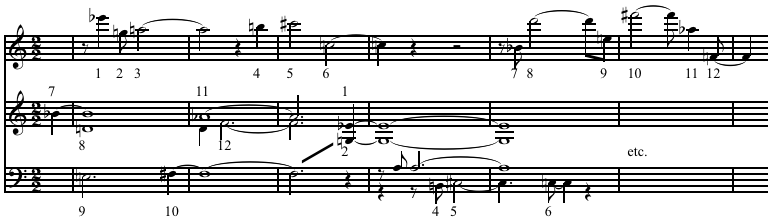
\includegraphics[width=\textwidth]{img/Schoenberg_-_Wind_Quintet_opening.png}
\caption{Ejemplo de composición con la serie dividida en voces\cite{wiki:twelvetonetechnique}} \label{fig:twelvetoneexample}
\end{figure}


\nocite{*}
\cleardoublepage
\addcontentsline{toc}{chapter}{Bibliografía}
\bibliographystyle{ieeetr}
\bibliography{bibliography}

\appendix
\chapter{Configuración del entorno}\label{aped.A}
Dado que sólo dispongo de medios con GNU/Linux y Windows 7 para probar el proyecto y el paquete de GNU/Linux está aún en fase alpha/beta a fecha de hoy, se explica en este apéndice la configuración del proyecto para el asistente y la librería de la que depende sobre Windows 7.

Accedemos a la página del IRCAM donde están los binarios para descargar: \url{http://forumnet.ircam.fr/shop/fr/forumnet/43-openmusic.html}

Instalamos el paquete con el asistente de instalación. En caso de no tener instalado Python, procedemos a descargarlo de su página web e instalarlo: \url{https://www.python.org/downloads/}

Descomprimimos el código y veremos que en la raíz está el fichero \emph{RuleTranslator.py}. Se ejecuta (por terminal o con doble click si está convenientemente configurado por el instalador de Python) y podemos exportar unos datos de prueba. Podemos cerrar la interfaz para configurar OpenMusic.

Abrimos OpenMusic y podemos elegir entre crear nuestro ``workspace'' o abrir uno ya existente. Si abrimos el que hemos descomprimido no hay que configurar nada. Vamos a explicar cómo configurar nuestro proyecto suponiendo que tenemos un ``workspace'' alternativo o uno nuevo.

Cuando tengamos nuestro ``workspace'' abierto vamos a configurar la librería de la que depende el asistente. Podemos dirigir OpenMusic a la carpeta del proyecto descomprimido o copiar la librería a nuestro ``workspace'' y dirigir OM ahí. De cualquier manera, la librería está en la carpeta \emph{TFG OM workspace/libraries}. En OpenMusic las librerías de usuario se añaden abriendo en el menú contextual \emph{OM 6.8/Preferences} y añadiendo la ruta donde está la librería y luego seleccionando el checkbox, tal y como se muestra en la imagen \ref{fig:configom}


\begin{figure}
\centering
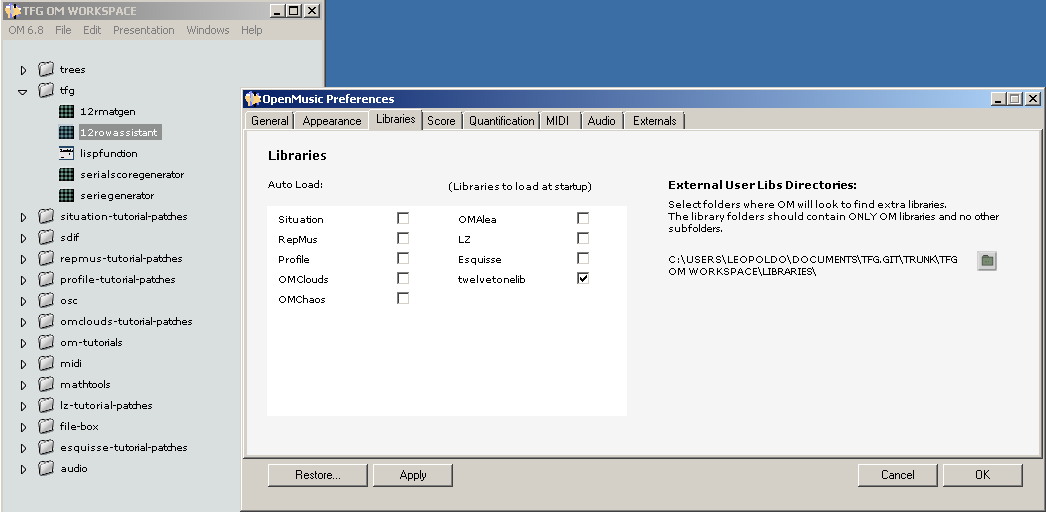
\includegraphics[width=\textwidth]{img/configom.png}
\caption{Ejemplo de composición con la serie dividida en voces} \label{fig:configom}
\end{figure}

Copiamos los ficheros de \emph{TFG OM workspace/in-files} que son los generados por la interfaz y los movemos a la carpeta in-files de nuestro ``workspace''. Ahora tan sólo tenemos que copiar los ``patches'' que forman el asistente, que están en la carpeta \emph{TFG OM workspace/elements/TFG}. Copiando la carpeta TFG en la carpeta elements de nuestro ``workspace'' será suficiente para que al reiniciar OpenMusic, detecte los nuevos ``patches''.

De esta forma, conseguimos cargar el proyecto del asistente en nuestro ``workspace'' y utilizarlo, modificarlo o crear un asistente derivado en un entorno diferente al adjunto.


\end{document}
